\documentclass{standalone}
\usepackage[x11names]{xcolor}
\usepackage{tikz}
\usetikzlibrary{calc}
\usetikzlibrary{arrows.meta}
\usetikzlibrary{decorations.pathmorphing}
\usetikzlibrary{decorations.pathreplacing}
\tikzset{sdot/.style = {fill, circle, inner sep = 1.5pt}}

\begin{document}
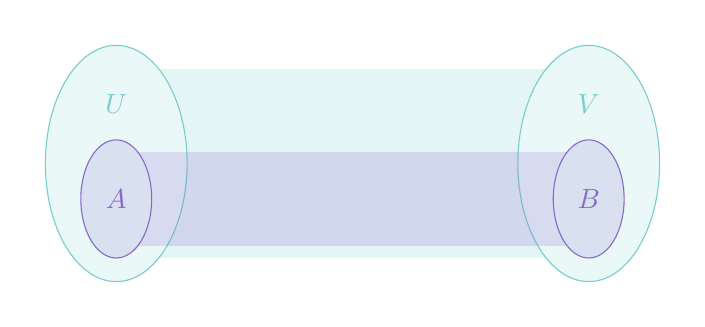
\begin{tikzpicture}[scale = 1.5]
    \fill [white] (-2.75, -1.15) rectangle (2.75, 1.15);
    \fill [DarkSlateGray3!20] (-2, -0.8) rectangle (2, 0.8);
    \filldraw [fill = DarkSlateGray3!15, draw = DarkSlateGray3] (-2, 0) ellipse (0.6 and 1);
    \filldraw [fill = DarkSlateGray3!15, draw = DarkSlateGray3] (2, 0) ellipse (0.6 and 1);
    \node [DarkSlateGray3] at (-2, 0.5) {$U$};
    \node [DarkSlateGray3] at (2, 0.5) {$V$};
    \fill [MediumPurple3, opacity = 0.2] (-2, -0.7) rectangle (2, 0.1);
    \filldraw [fill = MediumPurple3!50!DarkSlateGray3!30, draw = MediumPurple3] (-2, -0.3) ellipse (0.3 and 0.5);
    \filldraw [fill = MediumPurple3!50!DarkSlateGray3!30, draw = MediumPurple3] (2, -0.3) ellipse (0.3 and 0.5);
    \node [MediumPurple3] at (-2, -0.3) {$A$};
    \node [MediumPurple3] at (2, -0.3) {$B$};
\end{tikzpicture}
\end{document}